\subsection{Auroral Optical Flow Estimation}\label{sec:of}
Previous efforts \citep{blixt2006} used an optical flow estimator directly to estimate parameters of finely structured aurora, including structures associated with inverted-V and Alfvénic driven aurora.
Robust flow estimators flag areas where constraints are broken \citep{black1996}.
However, auroral events of interest often have video SNR approaching zero, and typical optical flow techniques are highly sensitive to noise due to the spatial derivatives employed.
Typical optical flow algorithms assume high SNR video, and so robust estimator constraints will simply be broken throughout the video frames on non-bright auroral video. 

A general method applicable to auroral video of any SNR, and particularly low SNR in order to capture the most possible events with acceptable false alarm rate is needed.
We do \textit{not} want to rely on seeing strong backscatter in the ISR from turbulence as that would bias observations toward only those with strong ISR backscatter.
The key criterion is sensitivity at low false alarm rate for $\textrm{SNR}\ll 2$ aurora.
The filtering of section~\ref{sec:filtnoise} mitigates the worst of the noise, but additional post-processing steps are needed, particularly for low SNR auroral video.
Optical flow estimators \citep{hornschunck} have been implemented in numerous languages including Python \citep{hscode} along with associated morphological and filtering operations.
%FIXME consider specific examples of Black vs Horn-Schunk vs Lucas Kanade

A typical scientific camera is a power sensor array of $512 \times 512$ or more pixels with 16-bit ADCs yielding data numbers $\in [0..65535]$.
Quantum efficiencies in the 50\% range for sCMOS and 90\% range for EMCCD yield vast weak auroral SNR advantages over early 8-bit digital cameras and the 5..10\% quantum efficiency obtained from the pinnacle of digital-assisted emulsion plate analog imaging \citep{parker1993}.
Even the narrowest auroral arcs observed with a medium field of view, say $10^\circ$ will cover several pixels for the E-region aurora of interest.
For a $10^\circ$ FOV lens/camera pair, each pixel of a $512\times512$ pixel camera aimed at magnetic zenith has approximately $10/512 = 0.0195^\circ$ spacing/pixel.
A \unit[100]{m} wide auroral arc with peak intensity at \unit[110]{km} near magnetic zenith subtends $\tan^{-1}(0.1/110) = 0.0521^\circ$, so the camera would see about 3..5 pixels covered by this arc, considering the point spread function (PSF) of the optical system.
These values represent the typical HiST optical setup as denoted in Table~\ref{tab:camerareshist}.
\begin{table}\centering
\caption{HiST camera resolution parameters.}\label{tab:camerareshist}
    \begin{tabular}{cccc}
        \toprule
        camera & binned resolution (pixels) & resolution ($B_\perp$ meters) & frames/sec\\
        \midrule
        iXon 879 & $512 \times 512$ & 37.5 & 30  \\
        iXon 897 & $512 \times 512$ & 37.5 & 50 \\
        \bottomrule
    \end{tabular}
\end{table}

The DMC instrument uses an Andor Neo sCMOS camera with $2560 \times 2160$ pixels and a Marshall \unit[140]{mm} lens, yielding a $6^\circ \times 8^\circ$ FOV.
This implies resolution of $6/2160 = 0.00278^\circ$/pixel, so a \unit[100]{m} wide arc covers about 19..22 pixels, considering PSF.
The reduced sensitivity of the sCMOS camera is partially offset by binning, that is, grouping of adjacent pixels into macropixels.
The averaging of the i.i.d. noise across the pixels improves SNR to first order by a factor $\sqrt{B_xB_y}$ where $B_x, B_y$ are the binning factors along the columns and rows of the image sensor respectively.
Typically for DMC experiments, $4 \times 4$ binning was used, yielding videos with the characteristics of Table~\ref{tab:cameraresdmc}.
The other camera used for context in the DMC system is an Andor iXon with a Kowa lens yielding a $50^\circ$ FOV, with parameters in Table~\ref{tab:cameraresdmc}.
These parameters are experimentally determined as per section~\ref{sec:hist}, the specification sheets and software ratings must be derated for all-night auroral capture.
\begin{table}\centering
    \caption{DMC camera resolution parameters.}\label{tab:cameraresdmc}
    \begin{tabular}{cccc}
        \toprule
        camera & binned resolution (pixels) & resolution ($B_\perp$ meters) & frames/sec\\
        \midrule
        iXon 897 & $512 \times 512$ & 187.5 & 30  \\
        Neo & $640 \times 540$ & 21.3 & 50 \\
        Neo & $320 \times 270$ & 42.6 & 100 \\
        \bottomrule
    \end{tabular}
\end{table}

Spatial derivatives for noise-filtered auroral video have magnitude
\begin{equation}
0 \leq |D| \leq \max(I)
\end{equation}
where $\max(I)$ is the maximum intensity in an image pair.
Stars will also have spatial derivatives somewhat larger than aurora, defined by the PSF of the optical system and seeing conditions.
An example optical flow measurement is shown in Figure~\ref{fig:optflowdiff}.
\begin{figure}\centering
    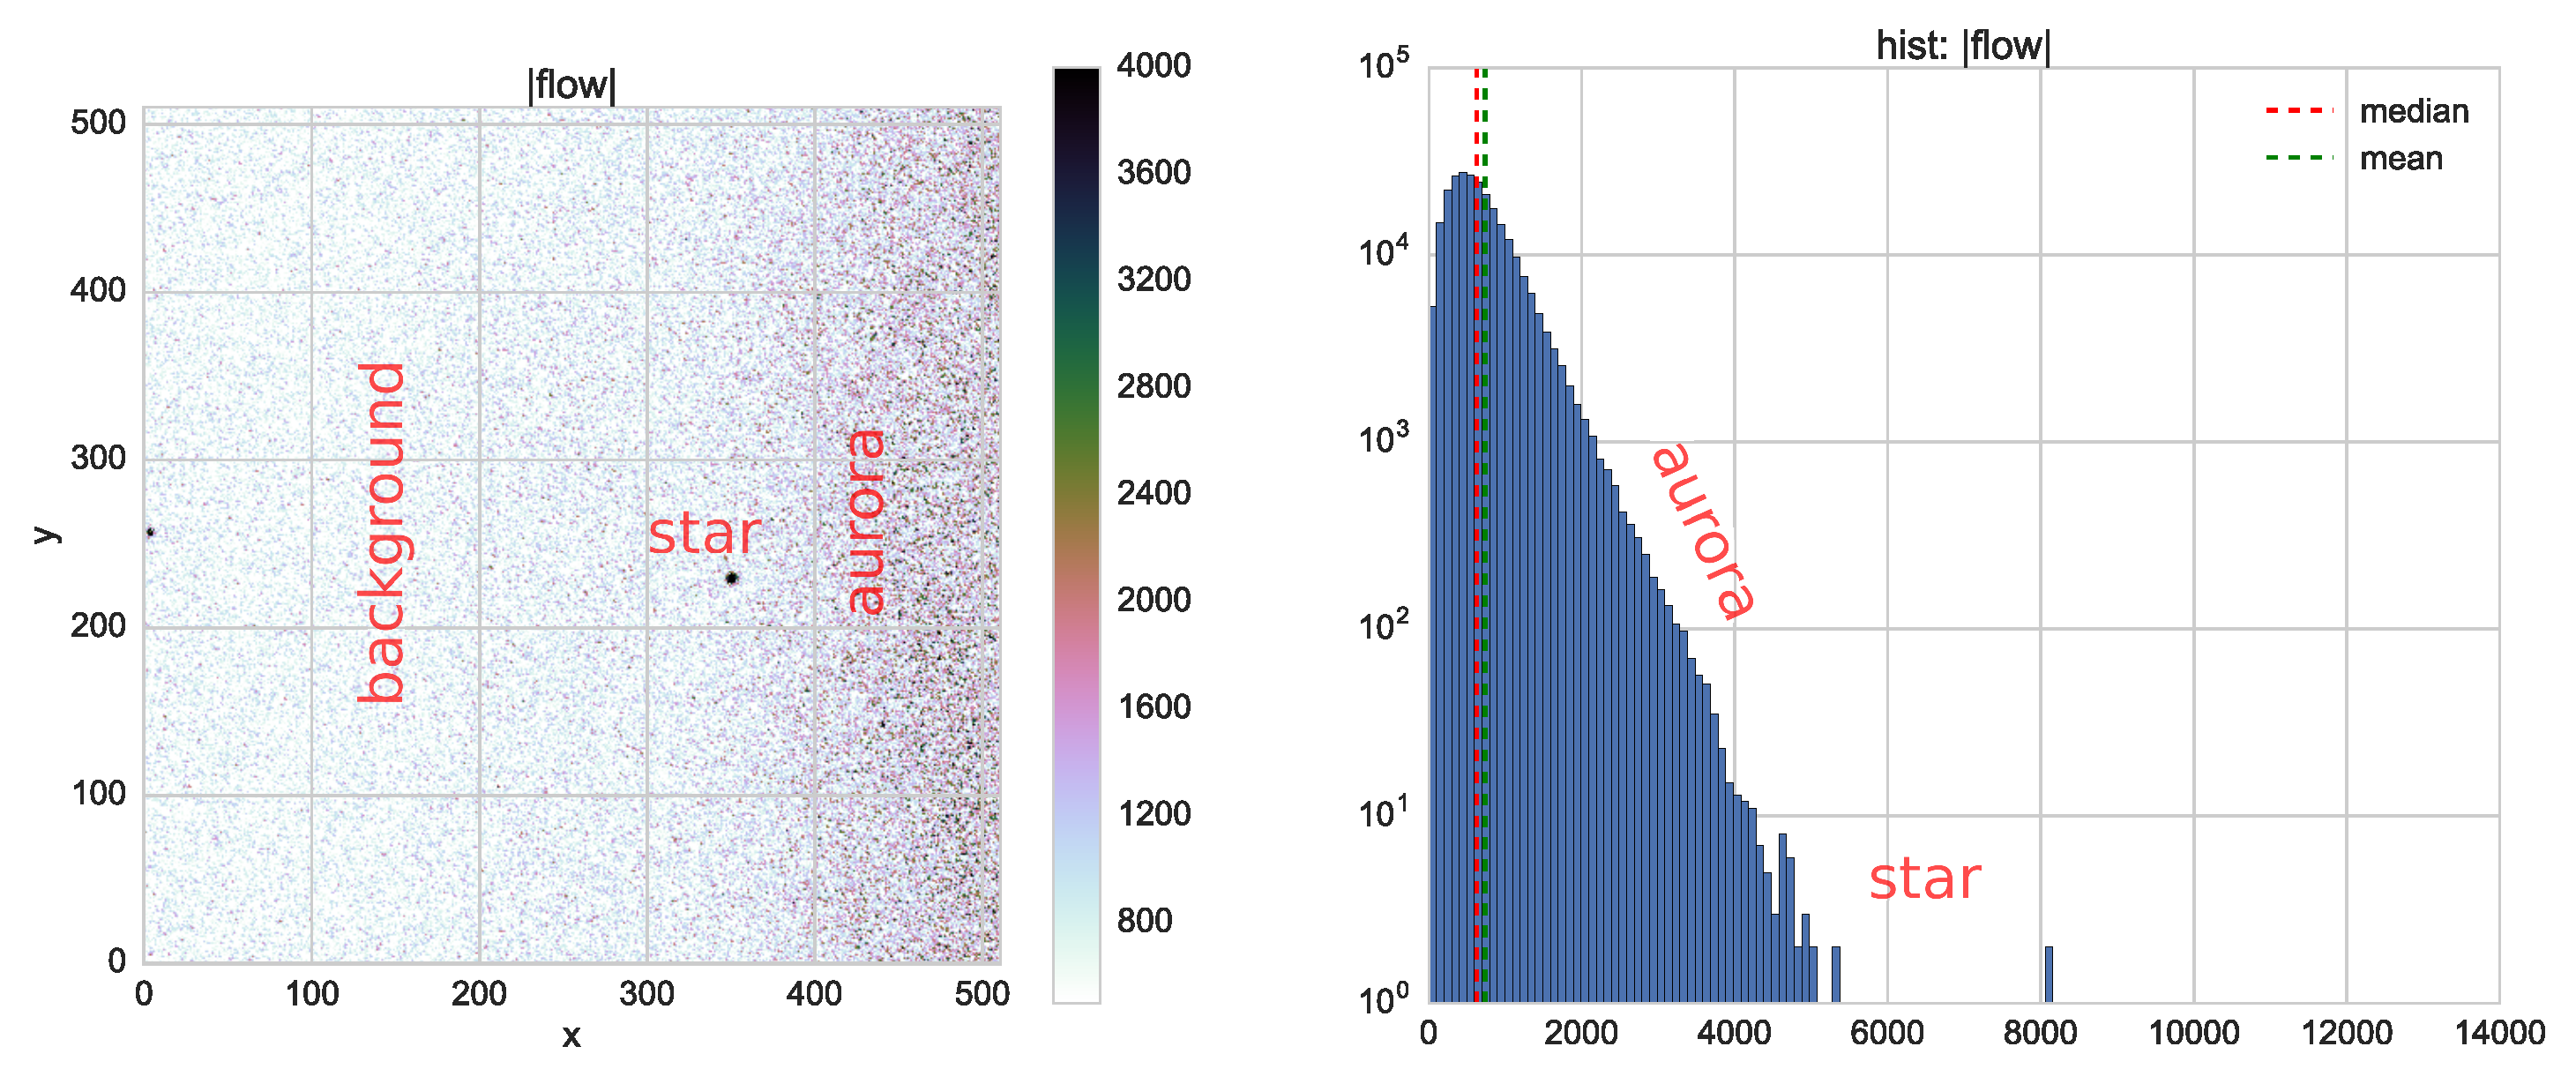
\includegraphics[width=\linewidth]{gfx/optflow-diffuse}
    \caption{(a) dense optical flow estimate using same image data as in Figure~\ref{fig:diffimhist}}\label{fig:optflowdiff}
\end{figure}
As with the image data histograms, the spatial derivative alone is not enough to distinguish interesting aurora from stars, clouds, and satellites.

Given the desire to exploit spatially correlated behavior of a discrete auroral arc, one typical approach is to reduce the resolution of the input image.
In this application however, to meet the spatial Nyquist criterion, we do not have the freedom to significantly reduce raw image resolution for risk of smearing out the closely spaced arcs that are vital to the purpose of HiST as seen by the parameters in Table~\ref{tab:camerareshist}.
Thus to exploit the locally collective behavior of aurora, particularly discrete aurora, optical flow estimation is chosen as a first processing step.
Farneback is a dense optical flow estimation algorithm that has proven suitable for the task.

%INWORK describe farneback parameters
The estimated optical flow $(U,V)$ is passed to the next module for segmentation.
